\documentclass[12pt, a4paper]{article}

\usepackage{graphicx}
\usepackage{amsmath}

\begin{document}

\tableofcontents
\newpage

\section{Problem 1 : Introduction}
\subsection{Description}

F5 : $ab^x$ is an exponential function, where a is a constant value, $a \ne 0$ and it also represents starting (initial) value , b is called base and is a positive real number and $b \ne 1$, x is called the exponent (power), it is independent variable . In this function, b is a constant value, whereas x is variable.

\subsection{Domain}

The domain for exponential function is the set of real numbers. 
\newline $x \in R$ ,  -$\infty < x <\infty$ , Domain : $\{x \mid x \in R$\}

\subsection{Co-Domain}

Co-Domain is the set of all possible function output values.
\newline Suppose $y = f(x) = ab^x $, then -$\infty < y <\infty$ , so the range will be $[-\infty,\infty]$.

\subsection{Characteristics}
\begin{itemize}
    \item In exponential function, if $ b > 0 $, then it is known as exponential growth function (increasing function). Its graphical representation shown in the left part of the figure 1.
    \item In exponential function, if $ 0 < b < 1$, then it is known as exponential decay function (decreasing function). Its graphical representation shown in the right part of the figure 1.
    \item Exponential function have horizontal asymptote (i.e function approaches to a imaginary horizontal line but never crosses) at $ Y=0 $ (i.e $ X $ – axis).
    \item They are continuous function.
    \item There is no symmetry in exponential function, so they are neither odd nor even function.
    \item Exponential function is not injective but is surjective. 
\end{itemize}

\newpage

\begin{figure}[h]
  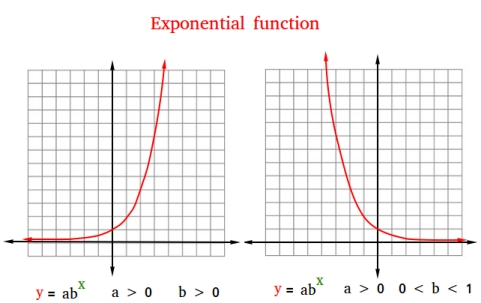
\includegraphics[width=\linewidth]{exponential-function.jpg}
  \caption{Exponential Function Graph (Growth And Decay).}
  \label{fig:exponential function graph (growth and decay)}
\end{figure}

\subsection{Context of Use Model}
\begin{figure}[h!]
  
\includegraphics[width=0.5\linewidth]{frog.jpg}
  \caption{Exponential Function Graph (Growth And Decay).}
  \label{fig:exponential function graph (growth and decay)}
\end{figure}


\newpage










\end{document}